\section{Language models}

\paragraph{Language model}
A language model is the probability distribution
of a sequence of words, it can be used for all sort 
of applications.
$$p(w_1, w_2, \dots, w_n)$$

\paragraph{Examples}
This probability could be used to predict the next word 
given a sequence
$$p(w_n | w_1, w_2, \dots, w_{n-1})$$
Another usage is to predict a feature given the sequence, 
for instance find the author from the text 
$$p(\mathit{author} | w_1, w_2, \dots, w_n)$$

\paragraph{Bases and evaluation}
The goal of language modeling is to build a computational model of the 
language of an entity $X$, that can be any entity in a domain.

Language models are entirely \emph{data-driven}. In other terms, 
we need to train models on the right data. One of the disadvantages of 
this fact is that instead of modeling the language of $X$, we are modelling
the language of the \emph{documents about X}.

\subsection{N-grams models}
The easier way to estimate a sequence probability is to count 
frequencies, but that could be unfeasible. We discussed a similar approach 
in Section \vref{problangmodel} in \emph{Computing a sentence probability}.

\paragraph{Unigram models}
A first approach is to use word frequencies, 
the idea is to find the relative frequency of a word, by simply counting 
it in the corpus and use it to estimate
the probability of a sequence.
$$p(w_n, w_{n-1}\dots, w_1) = p(w_n)p(w_{n-1})\dots p(w_1)$$
Note that this approach does not take into consideration the sequence in 
any way, this is a \emph{Unigram model} .

These models might be useful to compare two documents, where we 
need to compare the probability of seeing a given word, 
or to find how much relevant is a given word for a document. 
We can do that by comparing the word probability in all the dataset and in the
single document.

\paragraph{Pointwise Mutual Information}
$$\mathit{pmi}(a,b) = \log\frac{p(a,b)}{p(a)p(b)} = \log \frac{p(a | b)}{p(a)} = \log\frac{p(b|a)}{p(b)}$$
We can set the two variables to the event of extracting the document $C$ from 
the corpus and the probability $w$ of extracting a given word. 
$$\mathit{pmi}(w, C) = \log\frac{p(w, C)}{p(w)p(C)}$$
By computing the \emph{pmi} for the same word and two different documents, 
we can compare the difference of relevance of a word for the two 
documents.

\paragraph{Chain rule}
We now want to consider the sequence instead of taking words independently 
as in the unigram model.
$$p(w_k | w_1, \dots, w_{k-1}) = 
\frac{\mathit{count}(w_1, \dots, w_{k-1}, w_k)}{\sum_w \mathit{count}(w_1, \dots, w_{k-1}, w)}$$ 
Basically to compute the probability of finding a given word 
after a sequence, we count how many times we observe the sequence with
that word, over the count of all other words after the sequence.

In practice, we can reduce a long sequence to a shorter one, for instance
of two or three words, to potentially have enough data to estimate the probability.

\subsection{Evaluation}

There are basically two ways of evaluating a language model:
\begin{itemize}
    \item \emph{Extrinsic evaluation} : embed the system in a real applications
    and measure improvement
    \item \emph{intrinsic evaluation} : define a metric and evaluate the 
    model independent from any application, this requires a training set and 
    a testing set, where the second must be different but consistent 
    with the language learned by the model
\end{itemize}


\paragraph{Perplexity}
In the case of intrinsic evaluation, the main idea
 is to check if the model fits the test data. 
This measure is called perplexity.
$$\mathit{pp}(T) = p(w_1, \dots, w_n)^{-\frac{1}{n}}$$
For a two-gram model the measure becomes:
$$\mathit{pp}(T)= \sqrt[n]{\prod_{i=1}^n \frac{1}{p(w_i\;|\;w_{i-1})}}$$

\paragraph{Generalization and zero probabilities}
Language models have an issue when a word is present in the test set 
but not in the training set, this becomes unknown with no null probability.

To fix this we apply smoothing, for instance \emph{Laplace smoothing}, i.e. 
adding one to each word count, or a parameter k.

\paragraph{Backoff and interpolation}
Another way to deal with null probabilities 
is to apply \emph{backoff and interpolation}. Basically to estimate 
a $n$-gram frequency, if we do not have enough evidence, we use the $(n-1)$-gram 
frequency, until we have just a unigram.
An example can be:
$$p(\mathit{New\;York\;City}) = p(\mathit{City}\;|\;\mathit{York})\;p(\mathit{York}\;|\;\mathit{New}) $$

\emph{Interpolation} means computing a weighted sum over an $n$-gram levels, 
this way, even if we only observe the last word of a $n$-gram, we do not 
have zero probability.

\subsection{Word-Context models}
The problem of data sparsity is mitigated by the n-gram models, but not 
solved completely.

\paragraph{Skip-gram model}
The main of the model is to fix the cases where two sentences
are really similar, i.e. they give the same information, but they do 
not have any common n-gram.

We introduce the concept of \emph{word context}, 
basically we take a n-gram by skipping at most $k$ words, 
this leads to skip noisy terms.
By doing so, we could potentially match two sentences 
that differs for a few words but that do not share commons 
grams.

\paragraph{Continuous Bag of Words}
The idea of this model is to take the context of a word, 
for instance a collection of 2-grams, and predict a word.

\paragraph{Word context matrix}
We can think of a word context matrix, where we 
store information about appearance of a word $w$ 
within $t$ other words.

Taking into account the word order depends on the focus of
the model, in language the order is important, in semantics
it is less relevant.

The context matrix stores in $c_{i, j}$ for each word $w_i$
how many times the word $w_j$ occurs in its context. 
If we consider the row of that matrix as a vector, two words 
are close in that space if they have a similar context.

After computing the matrix, we can factorize it with singular value 
decomposition to obtain a more compact representation.
A problem is that such a factorization has many zero terms, to 
fix it we can \emph{weighted matrix factorization}.

\subsection{Word embeddings}

\paragraph{Words as vectors}
Representing words as vectors, as we did with models previously, 
is a very efficient way to compute words similarity and 
represent documents as regions in the vector space.
An example of word as vectors can be found in the context matrix.

The goal is to obtain \emph{dense word vectors}, so with small dimensionality 
and with the absence of sparsity.

\paragraph{Distributional hypothesis}
In a real world scenario a word has a meaning, which is related 
to the object, or the concept it represent, in our case there is 
no such thing, so we must find a way to deal with this.

We can assume that words that appear in the same 
context have the same meaning.

\subsubsection{Neural network models}

A first example of using a neural network is 
to take as input an $n$-gram of a word $w$ and
as output the probability distribution over the next word.

We saw this concept in the previous section when talking about 
\emph{Continuous Bag of Words}.

Basically what the network is doing is to compute 
this function
$$f(w_t, \dots, w_{t-n+1}) = P(w_t \; | \; w_1, \dots, w_{t-1})$$

\paragraph{Decomposition}
The idea used by the model is to decompose the function in 
two parts:
\begin{itemize}
    \item A mapping from any word $w_i \in V$ to a vector $w_i \in \mathbb{R}^m$ dimensions,
    this creates a matrix $W \in \mathbb{R}^{V \times m}$, where $V$ is the number of words
    \item A probability function over words, that takes in input 
    a sequence of vectors of $d$ dimensions, obtained via the previous
    mapping, and produces a vector $g$ in the original $V$ space.
\end{itemize}

\paragraph{Why is this relevant for word embeddings?}
The mapping to a $d$ dimensional space could be the word 
embedding we want to obtain, we are not interested 
in the network output.

We are assuming that the embedding made by the network 
correspond to the real meaning of the word, as such a 
mapping is obtained minimizing the objective function. 

In other words, if the network is able to perform well, that should 
be a good embedding.

\paragraph{Word2vec}
The idea is to train the neural network with positive couples of 
words and negative ones, with the hope the network will learn 
to output good words sequences.

The structure of the network in this implementation 
has an input and output layer of dimensions $V \times V$, 
and a middle layer of $V \times m$, initialized with random values.

After training we discard the output layer and keep the 
middle one, as discussed in the previous section.
The main principle is that similar vectors in the hidden 
layer corresponds to words with similar context. 

This is due to the fact that two words with the same context
should have similar consequent predictions, thus, the weights in 
the middle layer for this two words must be close, as the 
prediction made by the network must be more o less the same for 
the twos.

\begin{figure}[h]
    \centering
    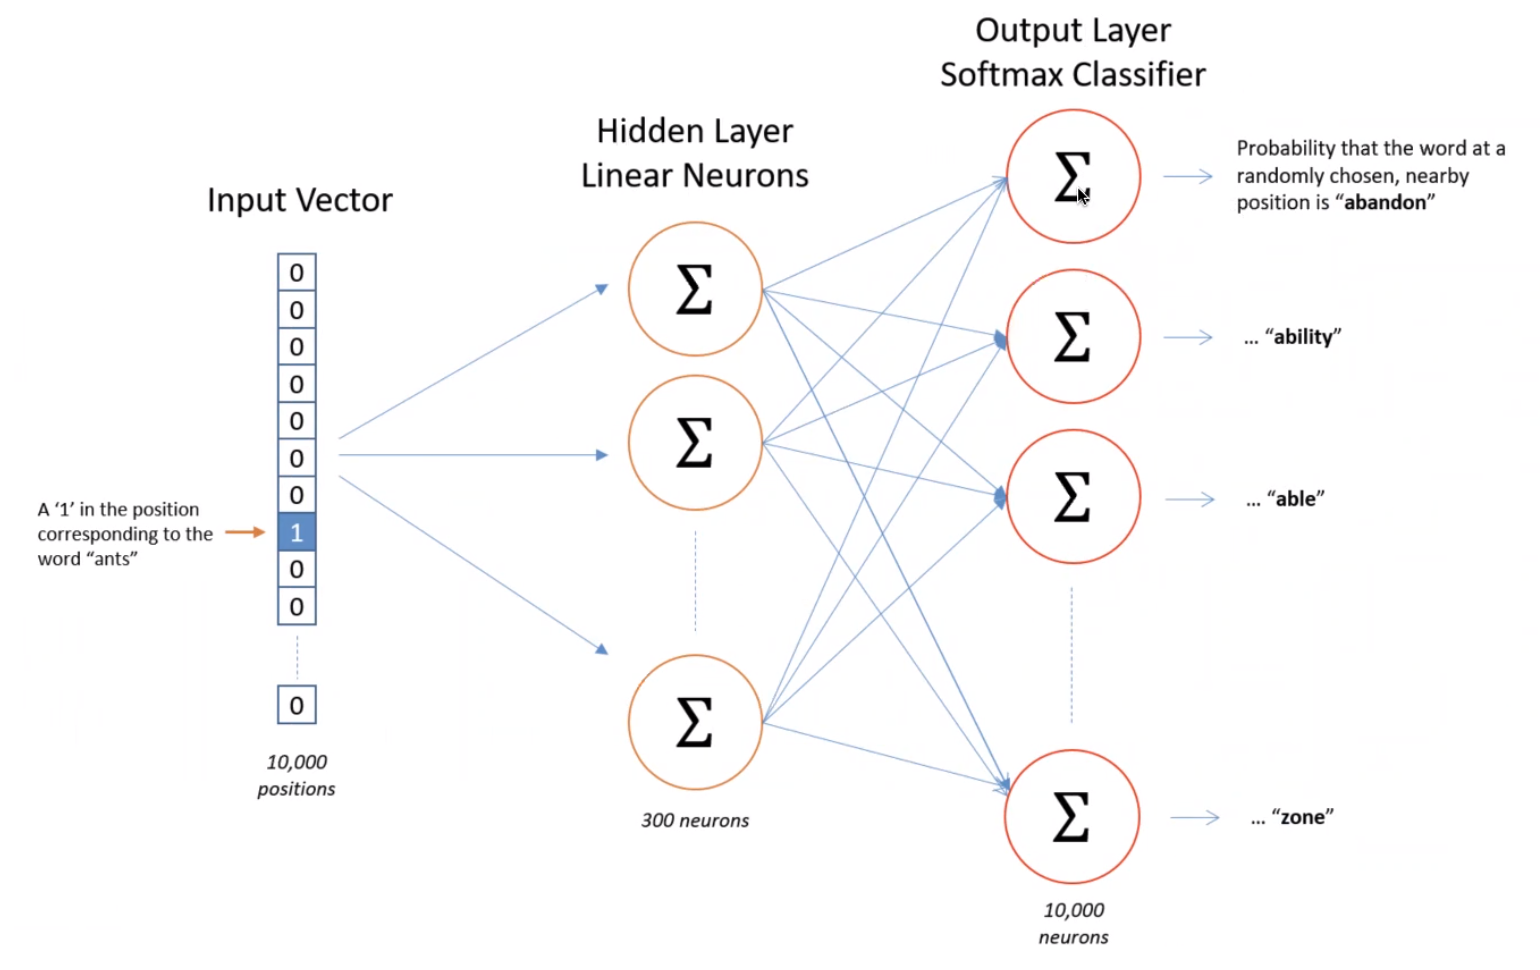
\includegraphics[width=0.8\textwidth]{images/nn-words.png}
    \caption{Word2vec implementation of Neural Network embedding}
\end{figure}

\subsubsection{Using embeddings}

\paragraph{Adding information}
We can use the word embeddings obtained in some way to improve 
retrieval, for instance by applying query expansion.

\paragraph{Similarity}
We can also compute similarity among group of words, 
as we have a vector space where for instance cosine similarity is 
applicable.